% !TEX root =  master.tex
\chapter{Anhang}


\subsubsection{Python Code zur Validierung der L"osbarkeit von Instanzen des 15-Puzzles}
\label{ssec:appendix-latency-benchmark}
\begin{lstlisting}[caption={Python Code zur Validierung der L"osbarkeit von Instanzen des 15-Puzzles}, label={code:validate-15-puzzle:py}]
\end{lstlisting}
\inputminted[linenos,breaklines,breakanywhere]{python}{../code/15-solvable.py}
\newpage

\subsubsection{Testing Output der verschiedenen Startzust\"ande}
\begin{figure}[H]
    \centering
    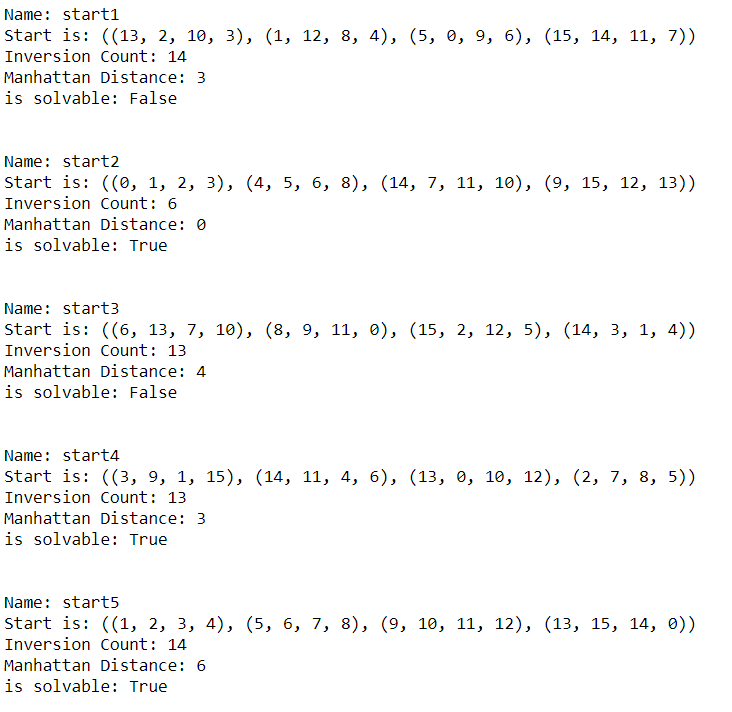
\includegraphics[width=\linewidth,keepaspectratio]{img/testing_output.PNG}
    \captionsetup{format=plain, indention=0pt}
    \caption{Testing Output der verschiedenen Startzust"ande \label{app:fig:testing-output}}
\end{figure}

\subsubsection{Puzzleinstanz mit hoher L"osbarkeitsberechnungsdauer}
\begin{figure}[H]
    \centering
    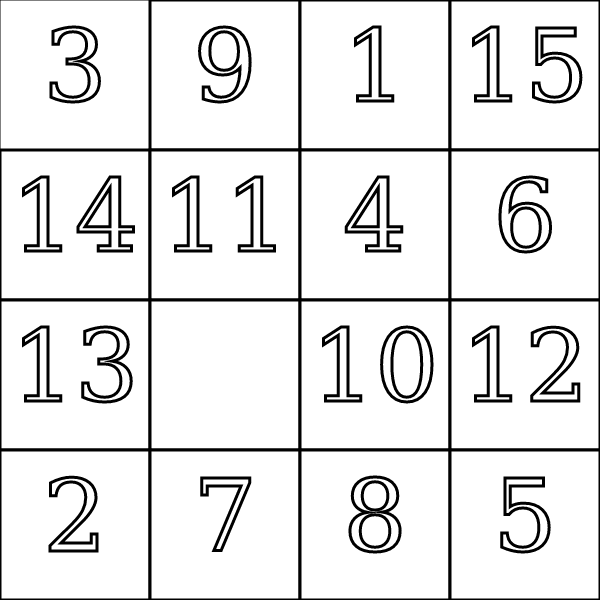
\includegraphics[width=0.5\linewidth,keepaspectratio]{img/time_consuming_puzzle_instance.png}
    \captionsetup{format=plain, indention=0pt}
    \caption{L"osbarkeitsberechnungsdauer \label{app:fig:time_c_p_i}}
\end{figure}

\subsubsection{Exemplarisches L"osen der in \ref{app:fig:time_c_p_i} angegebenen Puzzleinstanz (1h)}
\begin{figure}[H]
    \centering
    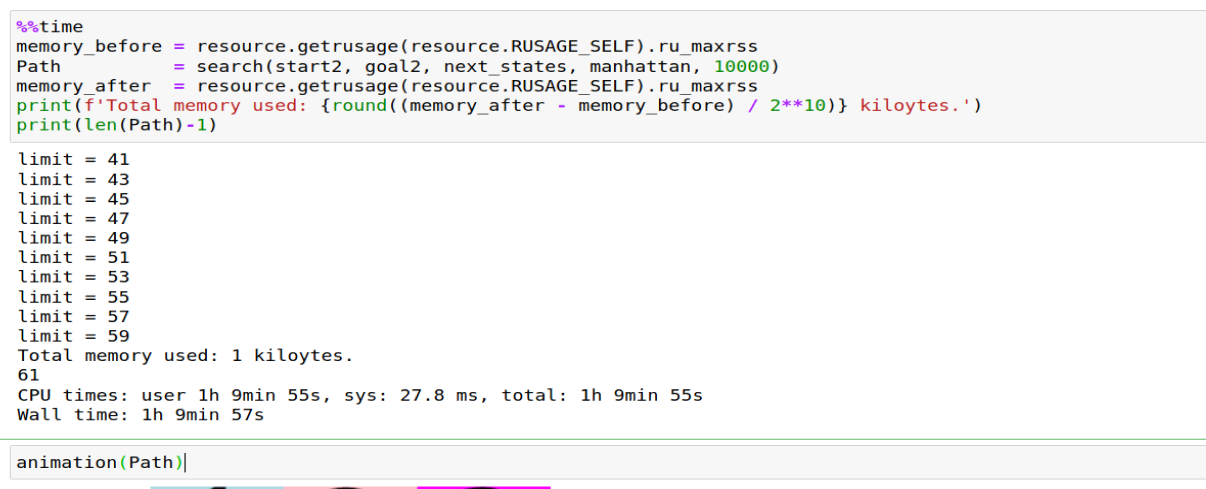
\includegraphics[width=\linewidth,keepaspectratio]{img/1h_solving_time_15_puzzle.png}
    \captionsetup{format=plain, indention=0pt}
    \caption{Exemplarisches L"osen eines 15-Puzzles mit hohem Zeitaufwand (1h) \label{app:fig:1h}}
\end{figure}
